\section{Experiments}
\label{sec:experiments}
We focus on routing problems: we consider the TSP, two variants of the VRP, the Orienteering Problem and the (Stochastic) Prize Collecting TSP. These provide a range of different challenges, constraints and objectives and are \emph{traditionally solved by different algorithms}. For the Attention Model (AM), we adjust the input, mask, decoder context and objective function for each problem (see Appendix for details and data generation) and train on problem instances of $n=20$, 50 and 100 nodes. For all problems, we use \emph{the same hyperparameters}: those we found to work well on TSP.

\paragraph{Hyperparameters}
We initialize parameters $\text{Uniform}(-1/{\sqrt{d}}, 1/{\sqrt{d}})$, with $d$ the input dimension. Every epoch we process 2500 batches of 512 instances (except for VRP with $n=100$, where we use 2500 $\times$ 256 for memory constraints). For TSP, an epoch takes 5:30 minutes for $n=20$, 16:20 for $n=50$ (single GPU 1080Ti) and 27:30 for $n=100$ (on 2 1080Ti's). We train for 100 epochs using training data generated on the fly. We found training to be stable and results to be robust against different seeds, where only in one case (PCTSP with $n=20$) we had to restart training with a different seed because the run diverged. We use $N=3$ layers in the encoder, which we found is a good trade-off between quality of the results and computational complexity. We use a constant learning rate $\eta = 10^{-4}$. Training with a higher learning rate $\eta = 10^{-3}$ is possible and speeds up initial learning, but requires decay ($0.96$ per epoch) to converge and may be a bit more unstable. See Appendix \ref{sec:appendix_results_tsp}. With the rollout baseline, we use an exponential baseline ($\beta = 0.8$) during the first epoch, to stabilize initial learning, although in many cases learning also succeeds without this `warmup'. Our code in PyTorch \citep{paszke2017automatic} is publicly available.\footnote{\url{https://github.com/wouterkool/attention-learn-to-route}}

\paragraph{Decoding strategy and baselines}
For each problem, we report performance on 10000 test instances.
At test time we use \emph{greedy} decoding, where we select the best action (according to the model) at each step, or \emph{sampling}, where we sample 1280 solutions (in $<1$s on a single GPU) and report the best. More sampling improves solution quality at increased computation.
In Table \ref{tab:results_problems} we compare greedy decoding against baselines that also construct a single solution, and compare sampling against baselines that also consider multiple solutions, either via sampling or (local) search. For each problem, we also report the `best possible solution': either optimal via \citetalias{gurobi} (intractable for $n > 20$ except for TSP) or a problem specific state-of-the-art algorithm.

\paragraph{Run times}
Run times are important but hard to compare: they can vary by two orders of magnitude as a result of implementation (Python vs C++) and hardware (GPU vs CPU). We take a practical view and report the time it takes to solve the test set of 10000 instances, either on a single GPU (1080Ti) or 32 instances in parallel on a 32 virtual CPU system (2 $\times$ Xeon E5-2630). This is conservative: our model is parallelizable while most of the baselines are single thread CPU implementations which cannot parallelize when running individually. Also we note that after training our run time can likely be reduced by model compression \citep{hinton2015distilling}. In Table \ref{tab:results_problems} we do not report running times for the results which were reported by others as they are not directly comparable but we note that in general our model and implementation is fast: for instance \citet{bello2016neural} report 10.3s for sampling 1280 TSP solutions (K80 GPU) which we do in less than one second (on a 1080Ti). For most algorithms it is possible to trade off runtime for performance. As reporting full trade-off curves is impractical we tried to pick reasonable spots, reporting the fastest if results were similar or reporting results with different time limits (for example we use Gurobi with time limits as heuristic).

\begin{table}[ht!]
\vskip -6mm
\caption{Attention Model (AM) vs baselines. The gap \% is w.r.t. the best value across all methods.}
\label{tab:results_problems}
\centering
\footnotesize
\setlength{\tabcolsep}{0.35em}
\renewcommand{\arraystretch}{0.8}
\begin{tabular}{ll|rrr|rrr|rrr}
 & &  \multicolumn{3}{c|}{$n = 20$} & \multicolumn{3}{c|}{$n = 50$} & \multicolumn{3}{c}{$n = 100$} \\
 & Method &  \multicolumn{1}{c}{Obj.} & \multicolumn{1}{c}{Gap} & \multicolumn{1}{c|}{Time} & \multicolumn{1}{c}{Obj.} & \multicolumn{1}{c}{Gap} & \multicolumn{1}{c|}{Time} & \multicolumn{1}{c}{Obj.} & \multicolumn{1}{c}{Gap} & \multicolumn{1}{c}{Time} \\
\midrule
\midrule
\multirow{21}{*}{\rotatebox[origin=c]{90}{TSP}}
 &  Concorde  &  $3.84$ & $0.00 \%$ & (1m) & $5.70$ & $0.00 \%$ & (2m) & $7.76$ & $0.00 \%$ & (3m) \\
 &  LKH3  &  $3.84$ & $0.00 \%$ & (18s) & $5.70$ & $0.00 \%$ & (5m) & $7.76$ & $0.00 \%$ & (21m) \\
 &  Gurobi  &  $3.84$ & $0.00 \%$ & (7s) & $5.70$ & $0.00 \%$ & (2m) & $7.76$ & $0.00 \%$ & (17m) \\
 &  Gurobi (1s)  &  $3.84$ & $0.00 \%$ & (8s) & $5.70$ & $0.00 \%$ & (2m) & \multicolumn{3}{c}{-} \\
\cmidrule{2-11}
 &  Nearest Insertion  &  $4.33$ & $12.91 \%$ & (1s) & $6.78$ & $19.03 \%$ & (2s) & $9.46$ & $21.82 \%$ & (6s) \\
 &  Random Insertion  &  $4.00$ & $4.36 \%$ & (0s) & $6.13$ & $7.65 \%$ & (1s) & $8.52$ & $9.69 \%$ & (3s) \\
 &  Farthest Insertion  &  $3.93$ & $2.36 \%$ & (1s) & $6.01$ & $5.53 \%$ & (2s) & $8.35$ & $7.59 \%$ & (7s) \\
 &  Nearest Neighbor  &  $4.50$ & $17.23 \%$ & (0s) & $7.00$ & $22.94 \%$ & (0s) & $9.68$ & $24.73 \%$ & (0s) \\
 &  \citeauthor{vinyals2015pointer} (gr.)  &  $3.88$ & $1.15 \%$ &  & $7.66$ & $34.48 \%$ &  & \multicolumn{3}{c}{-} \\
 &  \citeauthor{bello2016neural} (gr.)  &  $3.89$ & $1.42 \%$ &  & $5.95$ & $4.46 \%$ &  & $8.30$ & $6.90 \%$ &  \\
 &  \citeauthor{dai2017learning}  &  $3.89$ & $1.42 \%$ &  & $5.99$ & $5.16 \%$ &  & $8.31$ & $7.03 \%$ &  \\
 &  \citeauthor{nowak2017note}  &  $3.93$ & $2.46 \%$ &  & \multicolumn{3}{c|}{-} & \multicolumn{3}{c}{-} \\
 &  EAN (greedy)  &  $3.86$ & $0.66 \%$ & (2m) & $5.92$ & $3.98 \%$ & (5m) & $8.42$ & $8.41 \%$ & (8m) \\
 &  AM (greedy)  &  $\mathbf{3.85}$ & $\mathbf{0.34 \%}$ & (0s) & $\mathbf{5.80}$ & $\mathbf{1.76 \%}$ & (2s) & $\mathbf{8.12}$ & $\mathbf{4.53 \%}$ & (6s) \\
\cmidrule{2-11}
 &  OR Tools  &  $3.85$ & $0.37 \%$ &  & $5.80$ & $1.83 \%$ &  & $7.99$ & $2.90 \%$ &  \\
 &  Chr.f. + 2OPT  &  $3.85$ & $0.37 \%$ &  & $5.79$ & $1.65 \%$ &  & \multicolumn{3}{c}{-} \\
 &  \citeauthor{bello2016neural} (s.)  &  \multicolumn{3}{c|}{-} & $5.75$ & $0.95 \%$ &  & $8.00$ & $3.03 \%$ &  \\
 &  EAN (gr. + 2OPT)  &  $3.85$ & $0.42 \%$ & (4m) & $5.85$ & $2.77 \%$ & (26m) & $8.17$ & $5.21 \%$ & (3h) \\
 &  EAN (sampling)  &  $3.84$ & $0.11 \%$ & (5m) & $5.77$ & $1.28 \%$ & (17m) & $8.75$ & $12.70 \%$ & (56m) \\
 &  EAN (s. + 2OPT)  &  $3.84$ & $0.09 \%$ & (6m) & $5.75$ & $1.00 \%$ & (32m) & $8.12$ & $4.64 \%$ & (5h) \\
 &  AM (sampling)  &  $\mathbf{3.84}$ & $\mathbf{0.08 \%}$ & (5m) & $\mathbf{5.73}$ & $\mathbf{0.52 \%}$ & (24m) & $\mathbf{7.94}$ & $\mathbf{2.26 \%}$ & (1h) \\
\midrule
\midrule
\multirow{9}{*}{\rotatebox[origin=c]{90}{CVRP}}
 &  Gurobi  &  $6.10$ & $0.00 \%$ &  & \multicolumn{3}{c|}{-} & \multicolumn{3}{c}{-} \\
 &  LKH3  &  $6.14$ & $0.58 \%$ & (2h) & $10.38$ & $0.00 \%$ & (7h) & $15.65$ & $0.00 \%$ & (13h) \\
\cmidrule{2-11}
 &  RL (greedy)  &  $6.59$ & $8.03 \%$ &  & $11.39$ & $9.78 \%$ &  & $17.23$ & $10.12 \%$ &  \\
 &  AM (greedy)  &  $\mathbf{6.40}$ & $\mathbf{4.97 \%}$ & (1s) & $\mathbf{10.98}$ & $\mathbf{5.86 \%}$ & (3s) & $\mathbf{16.80}$ & $\mathbf{7.34 \%}$ & (8s) \\
\cmidrule{2-11}
 &  RL (beam 10)  &  $6.40$ & $4.92 \%$ &  & $11.15$ & $7.46 \%$ &  & $16.96$ & $8.39 \%$ &  \\
 &  Random CW  &  $6.81$ & $11.64 \%$ &  & $12.25$ & $18.07 \%$ &  & $18.96$ & $21.18 \%$ &  \\
 &  Random Sweep  &  $7.08$ & $16.07 \%$ &  & $12.96$ & $24.91 \%$ &  & $20.33$ & $29.93 \%$ &  \\
 &  OR Tools  &  $6.43$ & $5.41 \%$ &  & $11.31$ & $9.01 \%$ &  & $17.16$ & $9.67 \%$ &  \\
 &  AM (sampling)  &  $\mathbf{6.25}$ & $\mathbf{2.49 \%}$ & (6m) & $\mathbf{10.62}$ & $\mathbf{2.40 \%}$ & (28m) & $\mathbf{16.23}$ & $\mathbf{3.72 \%}$ & (2h) \\
\midrule
\midrule
\multirow{4}{*}{\rotatebox[origin=c]{90}{SDVRP}}
 &  RL (greedy)  &  $6.51$ & $4.19 \%$ &  & $11.32$ & $6.88 \%$ &  & $17.12$ & $5.23 \%$ &  \\
 &  AM (greedy)  &  $\mathbf{6.39}$ & $\mathbf{2.34 \%}$ & (1s) & $\mathbf{10.92}$ & $\mathbf{3.08 \%}$ & (4s) & $\mathbf{16.83}$ & $\mathbf{3.42 \%}$ & (11s) \\
\cmidrule{2-11}
 &  RL (beam 10)  &  $6.34$ & $1.47 \%$ &  & $11.08$ & $4.61 \%$ &  & $16.86$ & $3.63 \%$ &  \\
 &  AM (sampling)  &  $\mathbf{6.25}$ & $\mathbf{0.00 \%}$ & (9m) & $\mathbf{10.59}$ & $\mathbf{0.00 \%}$ & (42m) & $\mathbf{16.27}$ & $\mathbf{0.00 \%}$ & (3h) \\
\midrule
\midrule
\multirow{11}{*}{\rotatebox[origin=c]{90}{OP (distance)}}
 &  Gurobi  &  $5.39$ & $0.00 \%$ & (16m) & \multicolumn{3}{c|}{-} & \multicolumn{3}{c}{-} \\
 &  Gurobi (1s)  &  $4.62$ & $14.22 \%$ & (4m) & $1.29$ & $92.03 \%$ & (6m) & $0.58$ & $98.25 \%$ & (7m) \\
 &  Gurobi (10s)  &  $5.37$ & $0.33 \%$ & (12m) & $10.96$ & $32.20 \%$ & (51m) & $1.34$ & $95.97 \%$ & (53m) \\
 &  Gurobi (30s)  &  $5.38$ & $0.05 \%$ & (14m) & $13.57$ & $16.09 \%$ & (2h) & $3.23$ & $90.28 \%$ & (3h) \\
 &  Compass  &  $5.37$ & $0.36 \%$ & (2m) & $16.17$ & $0.00 \%$ & (5m) & $33.19$ & $0.00 \%$ & (15m) \\
\cmidrule{2-11}
 &  Tsili (greedy)  &  $4.08$ & $24.25 \%$ & (4s) & $12.46$ & $22.94 \%$ & (4s) & $25.69$ & $22.59 \%$ & (5s) \\
 &  AM (greedy)  &  $\mathbf{5.19}$ & $\mathbf{3.64 \%}$ & (0s) & $\mathbf{15.64}$ & $\mathbf{3.23 \%}$ & (1s) & $\mathbf{31.62}$ & $\mathbf{4.75 \%}$ & (5s) \\
\cmidrule{2-11}
 &  GA (Python)  &  $5.12$ & $4.88 \%$ & (10m) & $10.90$ & $32.59 \%$ & (1h) & $14.91$ & $55.08 \%$ & (5h) \\
 &  OR Tools (10s)  &  $4.09$ & $24.05 \%$ & (52m) & \multicolumn{3}{c|}{-} & \multicolumn{3}{c}{-} \\
 &  Tsili (sampling)  &  $5.30$ & $1.62 \%$ & (28s) & $15.50$ & $4.14 \%$ & (2m) & $30.52$ & $8.05 \%$ & (6m) \\
 &  AM (sampling)  &  $\mathbf{5.30}$ & $\mathbf{1.56 \%}$ & (4m) & $\mathbf{16.07}$ & $\mathbf{0.60 \%}$ & (16m) & $\mathbf{32.68}$ & $\mathbf{1.55 \%}$ & (53m) \\
\midrule
\midrule
\multirow{10}{*}{\rotatebox[origin=c]{90}{PCTSP}}
 &  Gurobi  &  $3.13$ & $0.00 \%$ & (2m) & \multicolumn{3}{c|}{-} & \multicolumn{3}{c}{-} \\
 &  Gurobi (1s)  &  $3.14$ & $0.07 \%$ & (1m) & \multicolumn{3}{c|}{-} & \multicolumn{3}{c}{-} \\
 &  Gurobi (10s)  &  $3.13$ & $0.00 \%$ & (2m) & $4.54$ & $1.36 \%$ & (32m) & \multicolumn{3}{c}{-} \\
 &  Gurobi (30s)  &  $3.13$ & $0.00 \%$ & (2m) & $4.48$ & $0.03 \%$ & (54m) & \multicolumn{3}{c}{-} \\
\cmidrule{2-11}
 &  AM (greedy)  &  $\mathbf{3.18}$ & $\mathbf{1.62 \%}$ & (0s) & $\mathbf{4.60}$ & $\mathbf{2.66 \%}$ & (2s) & $\mathbf{6.25}$ & $\mathbf{4.46 \%}$ & (5s) \\
\cmidrule{2-11}
 &  ILS (C++)  &  $3.16$ & $0.77 \%$ & (16m) & $4.50$ & $0.36 \%$ & (2h) & $\mathbf{5.98}$ & $\mathbf{0.00 \%}$ & (12h) \\
 &  OR Tools (10s)  &  $3.14$ & $0.05 \%$ & (52m) & $4.51$ & $0.70 \%$ & (52m) & $6.35$ & $6.21 \%$ & (52m) \\
 &  OR Tools (60s)  &  $\mathbf{3.13}$ & $\mathbf{0.01 \%}$ & (5h) & $\mathbf{4.48}$ & $\mathbf{0.00 \%}$ & (5h) & $6.07$ & $1.56 \%$ & (5h) \\
 &  ILS (Python 10x)  &  $5.21$ & $66.19 \%$ & (4m) & $12.51$ & $179.05 \%$ & (3m) & $23.98$ & $300.95 \%$ & (3m) \\
 &  AM (sampling)  &  $3.15$ & $0.45 \%$ & (5m) & $4.52$ & $0.74 \%$ & (19m) & $6.08$ & $1.67 \%$ & (1h) \\
\midrule
\midrule
\multirow{4}{*}{\rotatebox[origin=c]{90}{SPCTSP}}
 &  REOPT (all)  &  $3.34$ & $2.38 \%$ & (17m) & $4.68$ & $1.04 \%$ & (2h) & $6.22$ & $1.10 \%$ & (12h) \\
 &  REOPT (half)  &  $3.31$ & $1.38 \%$ & (25m) & $\mathbf{4.64}$ & $\mathbf{0.00 \%}$ & (3h) & $\mathbf{6.16}$ & $\mathbf{0.00 \%}$ & (16h) \\
 &  REOPT (first)  &  $3.31$ & $1.60 \%$ & (1h) & $4.66$ & $0.44 \%$ & (22h) & \multicolumn{3}{c}{-} \\
 &  AM (greedy)  &  $\mathbf{3.26}$ & $\mathbf{0.00 \%}$ & (0s) & $4.65$ & $0.33 \%$ & (2s) & $6.32$ & $2.69 \%$ & (5s) \\
\end{tabular}
\vskip -10mm
\end{table}
\subsection{Problems}

\paragraph{Travelling Salesman Problem (TSP)}
For the TSP, we report optimal results by Gurobi, as well as by Concorde \citep{concorde} (faster than Gurobi as it is specialized for TSP) and LKH3 \citep{helsgaun2017extension}, a state-of-the-art heuristic solver that empirically also finds optimal solutions in time comparable to Gurobi. We compare against Nearest, Random and Farthest Insertion, as well as Nearest Neighbor, which is the only non-learned baseline algorithm that also constructs a tour directly in order (i.e. is structurally similar to our model). For details, see Appendix \ref{sec:appendix_baselines}. Additionally we compare against the learned heuristics in Section \ref{sec:related_work}, most importantly \citet{bello2016neural}, as well as OR Tools reported by \citet{bello2016neural} and Christofides + 2OPT local search reported by \citet{vinyals2015pointer}. Results for \citet{dai2017learning} are (optimistically) computed from the \emph{optimality gaps} they report on 15-20, 40-50 and 50-100 node graphs, respectively. Using a \emph{single} greedy construction we outperform traditional baselines and we are able to achieve significantly closer to optimal results than previous learned heuristics (from around 1.5\% to 0.3\% above optimal for $n=20$). Naturally, the difference with \citet{bello2016neural} gets diluted when sampling many solutions (as with many samples even a random policy performs well), but we still obtain significantly better results, \emph{without} tuning the softmax temperature. For completeness, we also report results from running the Encode-Attend-Navigate (EAN) code\footnote{\url{https://github.com/MichelDeudon/encode-attend-navigate}} which is concurrent work by \citet{deudon2018learning} (for details see Appendix \ref{app:deudon}). Our model outperforms EAN, even if EAN is improved with 2OPT local search. Appendix \ref{sec:appendix_results_tsp} presents the results visually, including generalization results for different $n$.

\paragraph{Vehicle Routing Problem (VRP)}
In the Capacitated VRP (CVRP) \citep{toth2014vehicle}, each node has a demand and multiple routes should be constructed (starting and ending at the depot), such that the total demand of the nodes in each route does not exceed the vehicle capacity. We also consider the Split Delivery VRP (SDVRP), which allows to split customer demands over multiple routes. We implement the datasets described by \citet{nazari2018reinforcement} and compare against their Reinforcement Learning (RL) framework and the strongest baselines they report. Comparing greedy decoding, we obtain significantly better results. We cannot directly compare our sampling (1280 samples) to their beam search with size 10 (they do not report sampling or larger beam sizes), but note that our greedy method also outperforms their beam search in most (larger) cases, getting (in $<$1 second/instance) much closer to LKH3 \citep{helsgaun2017extension}, a state-of-the-art algorithm which found best known solutions to CVRP benchmarks. See Appendix \ref{sec:appendix_vrp_examples} for greedy example solution plots.

\paragraph{Orienteering Problem (OP)}
The OP \citep{golden1987orienteering} is an important problem used to model many real world problems. Each node has an associated \emph{prize}, and the goal is to construct a single tour (starting and ending at the depot) that \emph{maximizes} the sum of prizes of nodes visited while being shorter than a maximum (given) length. We consider the prize distributions proposed in \citet{fischetti1998solving}: \emph{constant}, \emph{uniform} (in Appendix \ref{sec:appendix_op_extended_results}), and increasing with the \emph{distance} to the depot, which we report here as this is the hardest problem. As `best possible solution' we report Gurobi (intractable for $n > 20$) and \emph{Compass}, the recent state-of-the-art Genetic Algorithm (GA) by \citet{kobeaga2018efficient}, which is only 2\% better than sampling 1280 solutions with our method (objective is maximization). We outperform a Python GA\footnote{\url{https://github.com/mc-ride/orienteering}} (which seems not to scale), as well the construction phase of the heuristic by \citet{tsiligirides1984heuristic} (comparing greedy or 1280 samples) which is structurally similar to the one learned by our model. OR Tools fails to find feasible solutions in a few percent of the cases for $n > 20$.

\paragraph{Prize Collecting TSP (PCTSP)}
In the PCTSP \citep{balas1989prize}, each node has not only an associated prize, but also an associated penalty. The goal is to collect at least a \emph{minimum} total prize, while minimizing the total tour length plus the sum of penalties of unvisited nodes. This problem is difficult as an algorithm has to trade off the penalty for not visiting a node with the marginal cost/tour length of visiting (which depends on the other nodes visited), while also satisfying the minimum total prize constraint. We compare against OR Tools with 10 or 60 seconds of local search, as well as open source C++\footnote{\url{https://github.com/jordanamecler/PCTSP}} and Python\footnote{\url{https://github.com/rafael2reis/salesman}} implementations of Iterated Local Search (ILS). Although the Attention Model does not find better solutions than OR Tools with 60s of local search, it finds almost equally good results in significantly less time. The results are also within 2\% of the C++ ILS algorithm (but obtained much faster), which was the best open-source algorithm for PCTSP we could find.

\paragraph{Stochastic PCTSP (SPCTSP)}
The Stochastic variant of the PCTSP (SPCTSP) we consider shows how our model can deal with uncertainty naturally. In the SPCTSP, the \emph{expected} node prize is known upfront, but the real collected prize only becomes known upon visitation. With penalties, this problem is a generalization of the stochastic k-TSP \citep{ene2018approximation}. Since our model constructs a tour one node at the time, we only need to use the real prizes to compute the remaining prize constraint. By contrast, any algorithm that selects a fixed tour may fail to satisfy the prize constraint so an algorithm \emph{must} be adaptive. As a baseline, we implement an algorithm that plans a tour, executes part of it and then re-optimizes using the C++ ILS algorithm. We either execute \emph{all} node visits (so planning additional nodes if the result does not satisfy the prize constraint), \emph{half} of the planned node visits (for $O(\log n)$ replanning iterations) or only the \emph{first} node visit, for maximum adaptivity. We observe that our model outperforms all baselines for $n = 20$. We think that failure to account for uncertainty (by the baselines) in the prize might result in the need to visit one or two additional nodes, which is relatively costly for small instances but relatively cheap for larger $n$. Still, our method is beneficial as it provides competitive solutions at a fraction of the computational cost, which is important in online settings.

\subsection{Attention Model vs. Pointer Network and different baselines}


\begin{wrapfigure}{R}{0.45\textwidth}
\vspace{-0.25in}
\begin{center}
\centerline{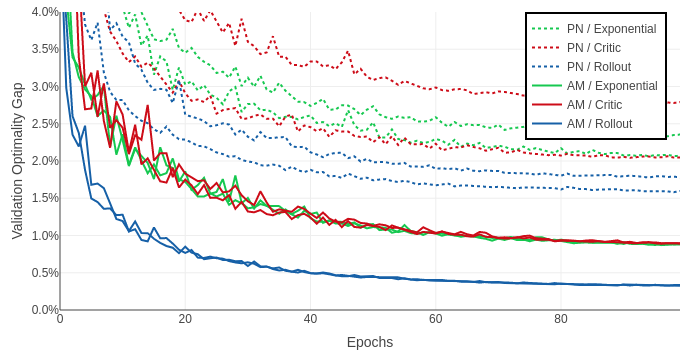
\includegraphics[width=\linewidth]{./images/baselines}}
\caption{Held-out validation set optimality gap as a function of the number of epochs for the Attention Model (AM) and Pointer Network (PN) with different baselines (two different seeds).}
\label{fig:progress}
\end{center}
\vskip -0.25in
\end{wrapfigure}
Figure \ref{fig:progress} compares the performance of the TSP20 Attention Model (AM) and our implementation of the Pointer Network (PN) during training. We use a validation set of size 10000 with greedy decoding, and compare to using an exponential ($\beta = 0.8$) and a critic (see Appendix \ref{sec:appendix_tsp_critic}) baseline. We used two random seeds and a decaying learning rate of $\eta = 10^{-3} \times 0.96^{\text{epoch}}$. This performs best for the PN, while for the AM results are similar to using $\eta = 10^{-4}$ (see Appendix \ref{sec:appendix_results_tsp}). This clearly illustrates how the improvement we obtain is the result of both the AM and the rollout baseline: the AM outperforms the PN using any baseline and the rollout baseline improves the quality and convergence speed for both AM and PN. For the PN with critic baseline, we are unable to reproduce the $1.5\%$ reported by \citet{bello2016neural} (also when using an LSTM based critic), but our reproduction is closer than others have reported~\citep{dai2017learning,nazari2018reinforcement}. In Table \ref{tab:results_problems} we compare against the original results. Compared to the rollout baseline, the exponential baseline is around 20\% faster per epoch, whereas the critic baseline is around 13\% slower (see Appendix \ref{sec:appendix_results_tsp}), so the picture does not change significantly if time is used as x-axis.